\section{Cycord Family}\label{sec:cycord}

Cycord calculi \citep{isli98_2doriordering} are based on oriented line segments,
either defined by a direction directly, or start and end point (cf.~dipoles in \ref{sec:dipole}).
The relations between two line segments $X$ and $Y$ can take one of the four values:
 $e$ (equal alignment), 
 $l$ (oriented left, i.e.~the angle $\alpha$ between $X$ and $Y$ is $\alpha\in(0,\pi)$, 
 $o$ (opposite, i.e.~$\alpha=\pi$, or
 $r$ (oriented right, i.e.~$\alpha\in(\pi,2\pi)$.
The binary case, where two oriented line segments are related, is equivalent to the alignment calculus (Section \ref{sec:geomoricalc}).
In the ternary case three line segments are considered and the relation consists of a three tuple
$(r_{XY},r_{XZ},r_{YZ})$
with
$r_{XY}$ denoting the binary relation between $X$ and $Y$,
$r_{XZ}$ between $X$ and $Z$, and
$r_{YZ})$ between $Y$ and $Z$.
Out of the 64 possible only 24 are valid, i.e.~only 24 are consistent in terms of the binary Cycord definition.

\subsection*{Binary CyCord}\label{sec:cycord-binary}

\kasten{
\subsubsection*{Binary Cycord calculus overview}
\begin{calcfeatures}
\feature{calculus identifier}{cycord2, cc2}
\feature{calculus parameters}{none}
\feature{arity}{binary}
\feature{entity type}{dipoles in the plane (oriented line segments)}
\feature{description}{relates two dipoles regarding their relative orientation (alignment)}
\feature{base relations}{e, l, o, r}
\lastfeature{references}{\citet{isli98_2doriordering}, \cite{isli00_2doriordering}}
%\feature{remarks]
\end{calcfeatures}
}
\begin{figure}[ht]
 	\centering
	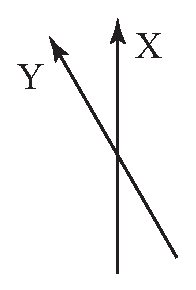
\includegraphics[width=0.15\textwidth]{cycord-binary}
	\caption{A binary Cycord relation: l}
	\label{fig:cc2}
\end{figure}

\subsection*{Ternary CyCord}\label{sec:cycord-binary}

\kasten{
\subsubsection*{Ternary Cycord calculus overview}
\begin{calcfeatures}
\feature{calculus identifier}{cycord3, cc3}
\feature{calculus parameters}{none}
\feature{arity}{ternary}
\feature{entity type}{dipoles in the plane (oriented line segments)}
\feature{description}{relates two dipoles regarding their relative orientation (alignment)}
\feature{base relations}{eee, ell, eoo, err, lel, lll, llo, llr, lor, lre, lrl, lrr, 
				     oeo, olr, ooe, orl, rer, rle, rll, rlr, rol, rrl, rro, rrr}
\lastfeature{references}{\citet{isli98_2doriordering}, \cite{isli00_2doriordering}}
%\feature{remarks]
\end{calcfeatures}
}
\begin{figure}[ht]
 	\centering
	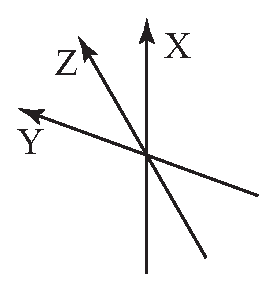
\includegraphics[width=0.15\textwidth]{cycord-ternary}
	\caption{A ternary Cycord relation: llr}
	\label{fig:cc3}
\end{figure}